\begin{figure}[ht] 
 	\centering 
 	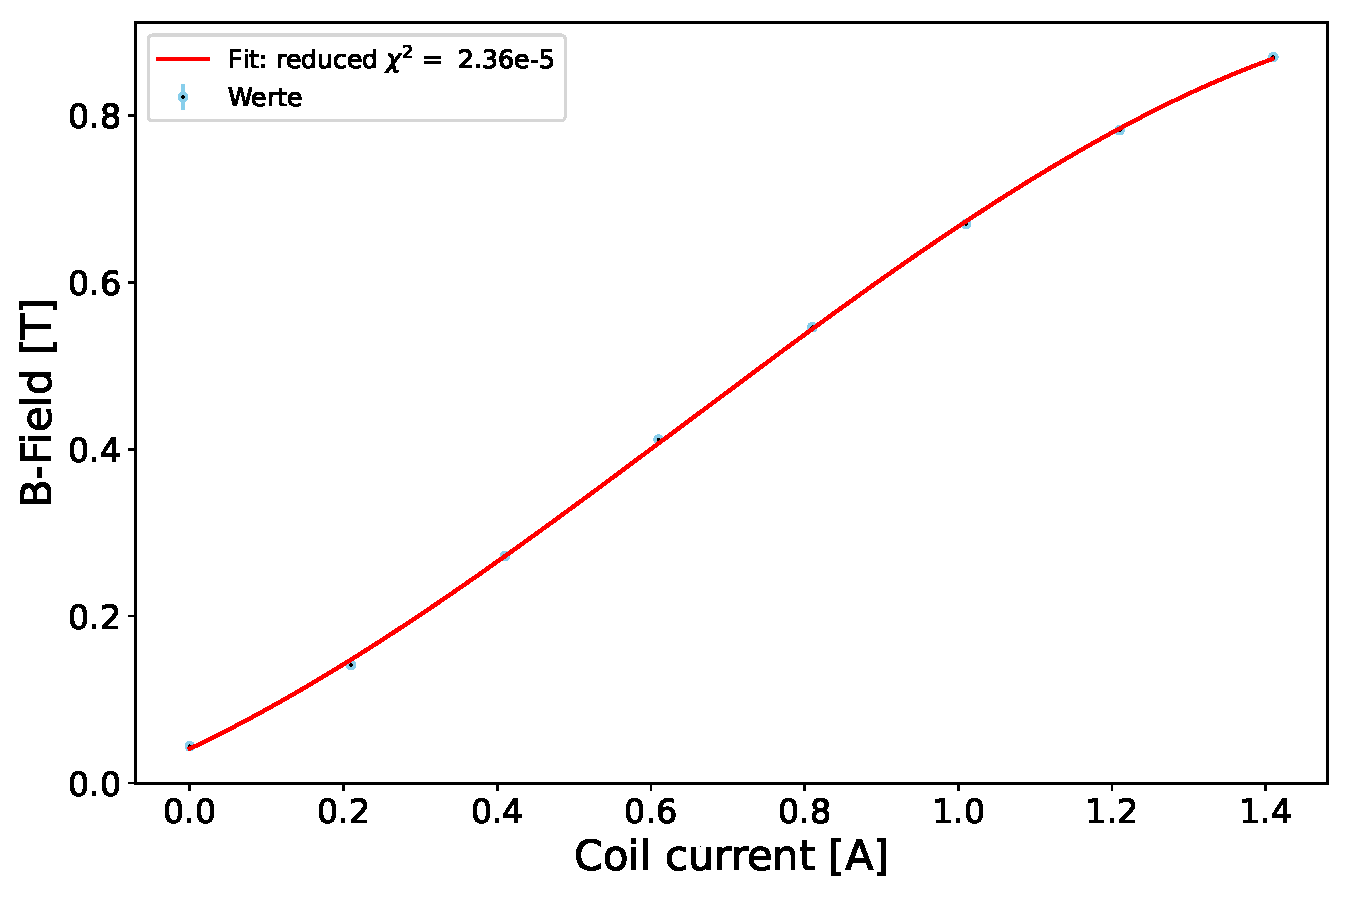
\includegraphics[width= 0.65 \textwidth]{Fits/B_field_Fit.pdf} 
	\caption{B_field, Fit} 
 	\label{fig:B_field, Fit} 
\end{figure}
 \\ 
\begin{table}[ht] 
\centering 
\caption{Amps_B06A, Fit Parameter Tabelle} 
\label{tab:my-table}
\begin{tabular}{|l|c|}
\hline
Parameter Name	&	Wert \\ \hline
c0	&	 0.041 \pm  0.00462\\ \hline
c1	&	 0.436 \pm  0.0303\\ \hline
c2	&	 0.394 \pm  0.0523\\ \hline
c3	&	-0.20335 \pm  0.0243\\ \hline
\end{tabular} 
\end{table}